\documentclass[12pt, a4paper]{report}
\usepackage{graphicx}
\usepackage{amsmath}
\usepackage{float}
\renewcommand{\baselinestretch}{1.2} 
\usepackage{ragged2e}
\usepackage{fancyvrb}
\usepackage{amssymb}
\usepackage[a4paper, total={7in, 9in}]{geometry}
\usepackage[utf8]{inputenc}
\usepackage{physics}
\usepackage{enumitem}


\title{\textbf{EE2703 : Applied Programming Lab \\ Assignment 6 \\ Tubelight Simulation}} % Title
\author{Arun Krishna A M S \\ EE19B001} % Author name
\date{\today} % Date for the report

\begin{document}		
		
\maketitle % Insert the title, author and date
\justifying

\section*{Aim}
In this assignment, we aim to understand how python helps in simulating models through:
\begin{itemize}
  	\item Simulating the one-dimensional model of tubelight
  	\item Plotting histograms for various graphs 
  	\item Vectorization of for-loops for faster computing
  	\item Plot the light intensity as a function of position (of tubelight) after the process has reached steady state
\end{itemize}

\section*{Introduction}

A uniform electric field accelerates the electrons present inside the tubelight.  Electrons are emitted from the cathode with zero energy, and accelerate in this field towards anode.  When they get beyond a threshold energy $E_0$, they can drive atoms to excited states. The relaxation of these collided atoms results in light emission. 

\textbf{Assumptions:}
\begin{itemize}
  	\item Relaxation of atoms after collision is instantaneous i.e., light emission is instantaneous
  	\item The tube-light is modelled as one-dimensional
  	\item Number of electrons introduced at cathode is normally distributed. 
  	\item Electrons come to rest after collision and accelerates again starting from zero velocity
\end{itemize}

\section*{Simulation}
We initialize the simulation universe as follows:
\begin{itemize}
  	\item The tube is divided in to a spatial grid of size \texttt{n} 
  	\item \texttt{m} electrons are injected from cathode at an average of \texttt{M} electrons with \texttt{Msig} standard deviation
  	\item Simulation is run for \texttt{nk} turns 
  	\item Electrons can excite the atoms only when they have velocities greater than \texttt{u0} with a probability \texttt{p} 
\end{itemize}
The default values are 
\begin{verbatim}
n    = 100     #spatial grid size.
M    = 5       #number of electrons injected per turn.
nk   = 500     #number of turns to simulate.
u0   = 5       #threshold velocity.
p    = 0.25    #probability that ionization will occur
Msig = 2       #deviation of elctrons injected per turn
\end{verbatim}
which can be changed based on user's input

Vectors of size \texttt{n*M} are created to store the Electron position \texttt{xx}, Electron velocity \texttt{u} and Displacement in each iteration \texttt{dx}. To hold the values for Intensity of emitted light \texttt{I}, Electron Position \texttt{X}, electron velocity \texttt{V}, lists are created since the length of these arrays are unknown beforehand. \\\\

\textbf{For each iteration (for \texttt{nk} times), We do the following:} \\

Find all the electrons present in the chamber: If the electron is present in the chamber, it must satisfy $0 < x < L = n$ between the cathode and the anode.
\begin{verbatim}
ii = np.where(xx > 0)[0]
\end{verbatim}
For these electrons which undergo acceleration, the values of position, velocity and displacement change. Assuming that the acceleration $a=1$ and with each iteration $\Delta t = 1$, we can say that
\begin{align*}
dx = \Delta x = u\Delta t + \frac{1}{2}a\Delta t^2 = u + 0.5\\
v = u + a\Delta t = u + 1\\
x = x + \Delta x = x + dx\\
 \end{align*}
Correspondingly the values are updated as follows:
\begin{verbatim}
dx[ii] = u[ii] + 0.5
xx[ii] += dx[ii]
u[ii] += + 1
\end{verbatim}
Determine the electrons that have hit the anode $x = L$ and set the positions, displacements and velocities of these particles to zero:
\begin{verbatim}
anodeReached = np.where(xx > n)[0]
xx[anodeReached] = 0
u[anodeReached] = 0
dx[anodeReached] = 0
\end{verbatim}
The electrons whose velocity is greater than threshold velocity is found 
\begin{verbatim}
kk = np.where(u >= u0)[0]                         
\end{verbatim}
These electrons have a probability \texttt{p} of colliding and ionizing the atom. The indices/location for these electrons are found and are stored in the \texttt{kl} variable
\begin{verbatim}
ll = np.where(np.random.rand(len(kk)) <= p)[0]    
kl = kk[ll]                                       
\end{verbatim}

These collisions would have occurred at any point between its previous known location $x_i[prev] = x_i - dx$ and current location $x_i$ i.e., the collision can occur any time in $(k-1) \Delta t < t < k \Delta t$. The collision of these electrons are uniformly distributed in time which means $t$ is uniformly distributed
\begin{verbatim}
t = np.random.rand(len(kl)) 
\end{verbatim}
Once the collision occurs, the velocity of electron becomes zero and it accelerates from that moment onwards. Note that only the accurate version is calculated here. Simple kinematics reveal that
\begin{verbatim}
xx[kl] = xx[kl] - dx[kl] + (u[kl]-1)*t + 0.5*t**2 + 0.5*(1-t)**2
u[kl] = 0 + (1-t)
\end{verbatim}
The excited atoms at this location resulted in emission from that point. So we have to add a photon at that point. 
\begin{verbatim}
I.extend(xx[kl].tolist())
\end{verbatim}
Normally distributed \texttt{m} electrons are injected from cathode at a mean of \texttt{M} electrons with $\sigma = $\texttt{Msig} standard deviation.
\begin{verbatim}
m = int(randn()*Msig + M)
\end{verbatim}
We now find the empty slots in \texttt{xx} array to add the newly injected electrons. If the number of electrons to be injected is greater than the available slots, then we add electrons only in those available empty slots. Note that there is no real-life significance of electrons greater than available slots since this doesn't happen in real life. Hence this is generally avoided by choosing \texttt{xx} array to hold sufficiently large number of values.\\
The electrons are generated very close to the cathode with zero initial velocity. 
\begin{verbatim}
emptySlots = np.where(xx==0)[0]
temp = min(m, len(emptySlots))
xx[emptySlots[:temp]] = 1 
u[emptySlots[:temp]]  = 0 
dx[emptySlots[:temp]] = 0 
\end{verbatim}

Again all the existing electrons are found. Their positions and velocities are added to \texttt{X} and \texttt{V} vectors
\begin{verbatim}
temp = np.where(xx > 0)[0]
X.extend(xx[temp].tolist())
V.extend(u[temp].tolist())
\end{verbatim}

\section*{Plot}
We observe the following histogram plots:

\begin{center}
	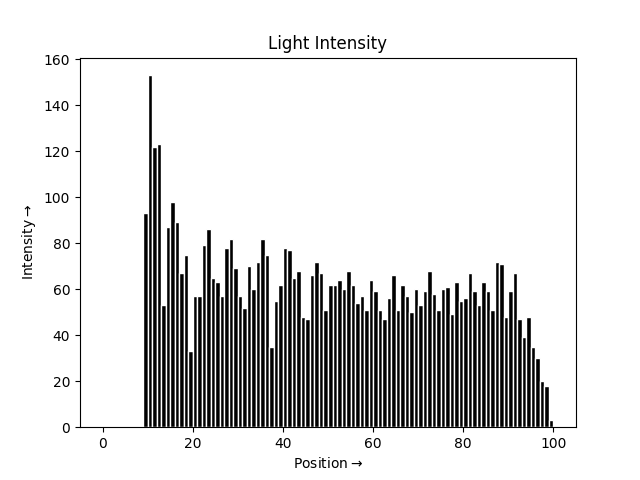
\includegraphics[scale=1]{Figure_0} 
	\label{fig:rawdata}
\end{center}
We can observe that the region upto 8 is where the electrons are building up the energy. Theoretically excitation cannot happen within this region $x < \frac{u_0^2}{2a} = < \frac{u_0^2}{2} = 12.5$, since the energy is not sufficient for the ionization of atoms.

\begin{center}
	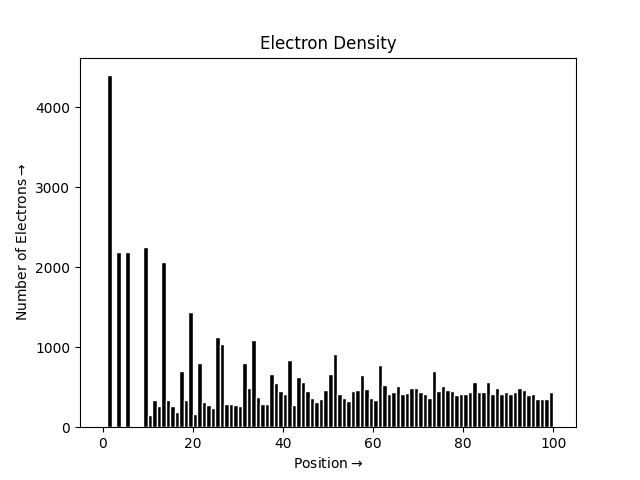
\includegraphics[scale=0.90]{Figure_1} 
	\label{fig:rawdata}
\end{center}

\begin{center}
	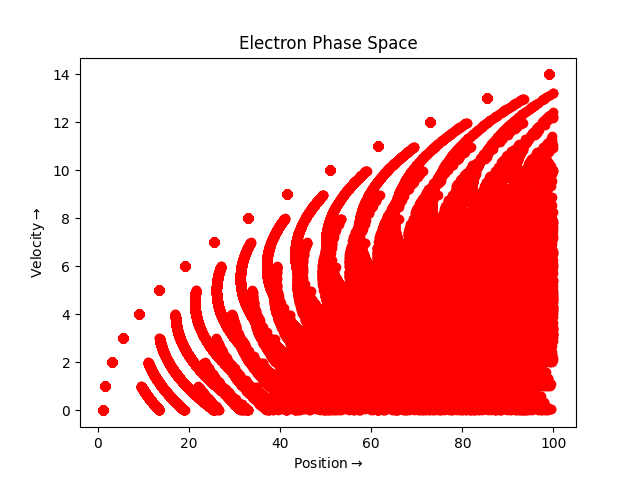
\includegraphics[scale=0.90]{Figure_2} 
	\label{fig:rawdata}
\end{center}
\clearpage
Tabulating Intensity vs Position:
\begin{center}
\begin{tabular}{ |c|c| } 
 \hline
xpos & count \\ 
0 & 0.0\\
1 & 0.0\\
2 & 0.0\\
3 & 0.0\\
4 & 0.0\\
5 & 0.0\\
6 & 0.0\\
7 & 0.0\\
8 & 0.0\\
9 & 105.0\\
10 & 157.0\\
11 & 160.0\\
12 & 136.0\\
13 & 60.0\\
14 & 126.0\\
15 & 89.0\\
16 & 105.0\\
17 & 103.0\\
. & . \\
. & . \\
. & . \\
. & . \\
. & . \\
. & . \\
89 & 70.0\\
90 & 66.0\\
91 & 66.0\\
92 & 51.0\\
93 & 49.0\\
94 & 39.0\\
95 & 37.0\\
96 & 41.0\\
97 & 20.0\\
98 & 14.0\\
99 & 7.0\\
 \hline
\end{tabular}
\end{center}



\section*{Inaccurate Solution}
An inaccurate simulation for this model would be to assume that the collisions are uniformly distributed in space instead of time. We obtain the actual point of collision and update the \texttt{xx} array like: $x_i \leftarrow x_i-dx_i \rho$ where $\rho$ is an uniformly distributed random number between 0 and 1.

\begin{verbatim}
xx[kl] = xx[kl] - dx[kl]*np.random.rand()
u[kl] = 0
\end{verbatim}
Following plot results can be observed:
\begin{center}
	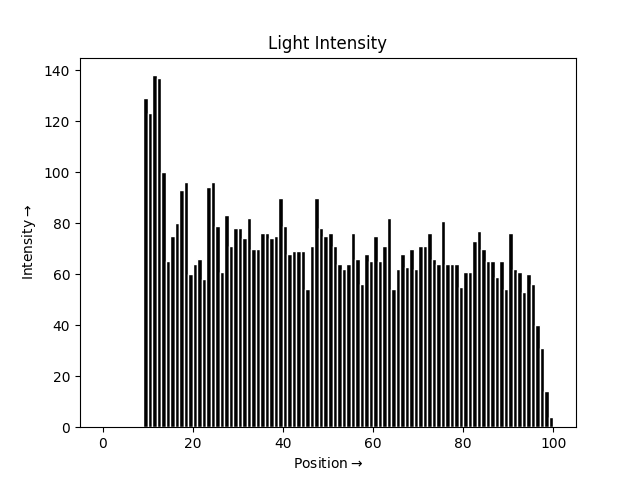
\includegraphics[scale=0.70]{Figure_4} 
	\label{fig:rawdata}
\end{center}
\begin{center}
	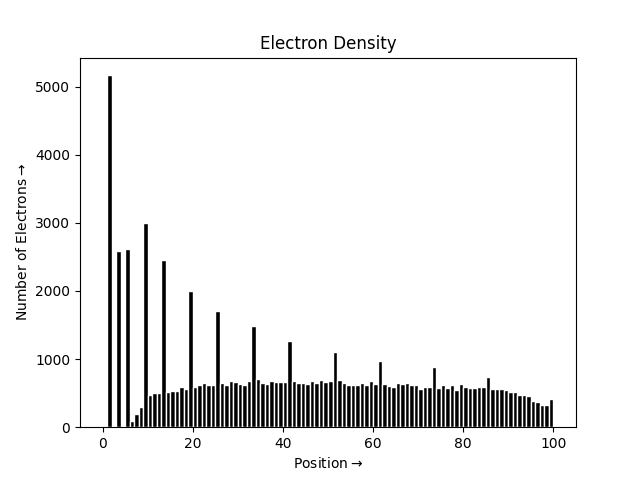
\includegraphics[scale=0.70]{Figure_5} 
	\label{fig:rawdata}
\end{center}
\begin{center}
	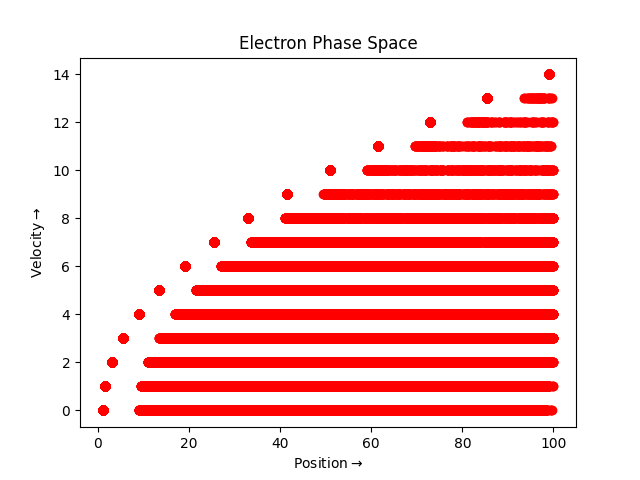
\includegraphics[scale=0.80]{Figure_6} 
	\label{fig:rawdata}
\end{center}

\section*{Conclusion}
An one-dimensional model of tubelight was made and simulated. Light intensity, Electron density and phase space diagrams were plotted for both the accurate and inaccurate depictions. We observed that the ionization of atoms didn't happen in the initial region, since the energy of the electron was not enough to cross the threshold voltage. Electron Phase Space diagram seems to have a profile of parabolic envelope for the accurate version indicating bands of electrons having same velocities
\end{document}

